\documentclass{article}
%\documentclass[aps,prb,twocolumn,superscriptaddress,floatfix]{revtex4}
\usepackage{graphicx}
\usepackage{epsfig}
\usepackage{amsmath}
\usepackage{amssymb}
\usepackage{subfig}
\usepackage{wrapfig}
\usepackage{mathptmx, microtype}
\usepackage[utf8]{inputenc}
\usepackage{xcolor, color, soul}
\sethlcolor{red}

\usepackage{hyperref}



\usepackage{titlesec}

\begin{document}
\frenchspacing




\title{Kickstarter Campaign - Games company}

\date{\today}

\author{Ovando Carter}

\maketitle

\newpage

\tableofcontents








\maketitle

\clearpage

\section{Brief Introduction}



\begin{itemize}
\item Small board game company’s first Kickstarter campaign.
\item Need a minimum of \$15,000 USD to get this project off the ground.
\item Wants to expand the business.
\item Would like to maximise our funding for this campaign.
\end{itemize}

\noindent The company would like data-driven recommendations to answer the following questions: 

\begin{enumerate}
\item What is a realistic Kickstarter campaign goal (in dollars) should the company aim to raise?
\item How many backers will be needed to meet their goal?
\item How many backers can the company realistically expect, based on trends in their category?
\end{enumerate}



\section{Preliminary Data Analysis}

\noindent The questions raised by the executives are given below. 

\begin{enumerate}
\item What are the names of the top 3 campaigns by the amount of money pledged?
\item Determine if the funding goal differs significantly between successful and failed campaigns.
\item Name the three countries that had the highest number of campaigns.
\item What is the average amount pledged per backer for successful campaigns?
\item How many sub-categories have an average per backer pledge greater than 250 dollars?.
\end{enumerate}

\noindent  the following are the results gained from use of SQL.

\medskip
\subsection{Top campaigns}

\subsubsection{Money Raised}
The top three campaigns  by the amount of money pledged are:

\noindent Based on the data we can see that kickstarter campaigns have a number of successful areas. The top three categories are, Technology, Games, and Design, which generated \$28.8 mil, \$28.3 mil, and \$23.8 mil, respectively. 

\medskip

\noindent For the subcategories, Product Design, Tabletop Games, and Video Games were the top three, having raised \$21.0 mil, \$19.3 mil and 7.8 mil, respectively. Notably, there are two games subcategories in this line up, however video games could also be considered technology. From this we can see that computer games generated only 40\% of that of table top games. This is a good indication that Tabletop Games are a more attractive area to pursue. 


\medskip

\noindent Gloomhaven (second printing) was a table top game that alone generated the highest pledged amount of \$3,999,795.77 with a total number of 40,642 backers. Thus giving an average of \$498.41 per backer. Again building confidence that a single table top game can support a strong campaign.  

\subsubsection{Backers}

\noindent The top campaigns by backers are Games, Technology and Design, with the number of backers totalling (411,671), (329,751), and (262,245), respectively. Again, Games and technology hold a similar number of supporters based on historical data. Both areas could support a successful campaign, however as mentioned earlier table top games generated considerably more income than their technology counterparts. Working on producing a table top game is again supported here. 

\medskip
\subsection{Funding goal \& campaigns}
\noindent Dose the funding goal differ significantly between successful and failed campaigns?

\noindent Shorter campaigns had an average pledge of \$9,086.19 which was only \$533.80 more than longer campaigns per pledge. However when considering the total amount generated at \$126.5 mil we can see that a larger amount of money is generated in shorter campaigns where longer campaigns only reached \$9.2 mil for the same data set. 

\subsubsection{Failed campaigns}
\noindent Notably, for the campaigns that failed, 7,330 of them where shorter ones, where as only 520 of them were longer ones. This is reflected again in the successful campaigns where in this case 4,990 of them were short while only 329 were longer. 

\medskip

\noindent Shorter campaigns appear more profitable and more economical than longer ones. 

\subsubsection{Successful campaigns} 
\noindent Longer campaigns has 15 times more short campaigns as they do loner ones. Again, the difference between the average plegde is not much, but again shorter campaigns generated more than their longer counterparts, at \$9,08


\medskip
\subsection{Top countries.}

The top three countries with the highest number of campaigns are:

\medskip

\begin{figure}[h]
\begin{center}
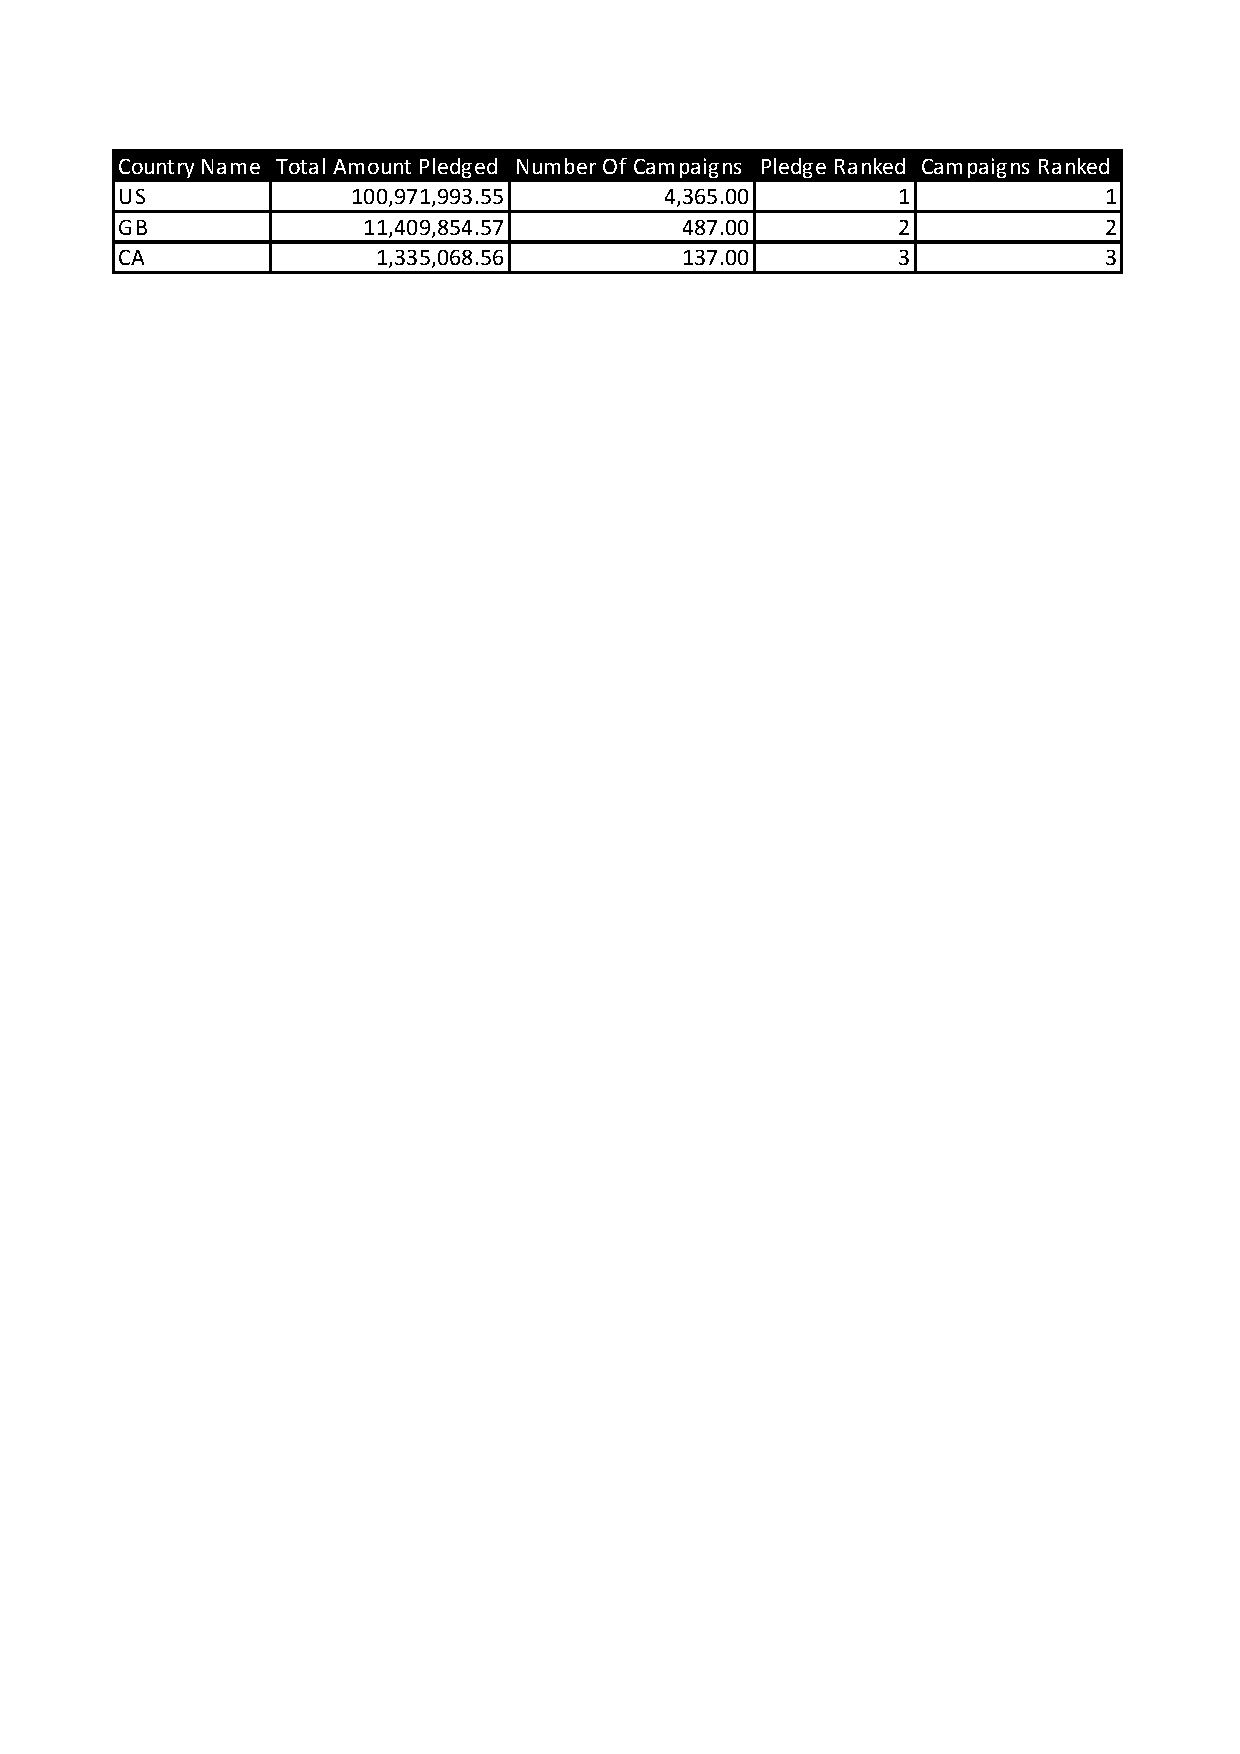
\includegraphics[width= 12 cm]{top-three-countries.pdf}
\end{center}
\caption{\label{fig:top-three-countries}  Top-3-countries by amount pledged and No. Campaigns}
\end{figure}

\noindent  As can be seen by Fig.~\ref{fig:top-three-countries}, the top three countries are the United States (US), Great Britain (GB), and Canada (CA).  With the US leading by far with 4,365 campaigns and 100,971,993.55 pledges. 

\medskip
\noindent The UK and CA only generating 11.16\%, and 3.15\% in pledges, respectively.

\medskip
\noindent Moreover, the US generated, 89,562,139, and 99,636,925 more pledges than that of GB and CA, respectively. Thus showing the US to be the biggest single market by far. 



\medskip

\noindent NB: One of the countries given was "N,0", as this was clearly not a county code it was changed to "unknown". This could be the result of a typo or corrupted data input. For this reason it was chosen that this data would not be included in the analysis. 

\medskip
\subsection{Average amount pledged}
\noindent The average amount pledged per backer for successful campaigns were,  \$268.00, \$170.38, and \$4150.00 for the subcategories Latin, Crochet and Glass, respectively. 

\medskip
\subsection{How many sub-categories}

The number of sub-categories that have an average per backer pledge greater than 250 dollars are:



\section{Conclusion}


\begin{itemize}
\item As their goal is \$15k, and the average pledge per backer in table top games is \$78.22, this would mean that the campaign requires only 192  backers to reach their goal. 
\item Based on trends in the table top games category, the average number of backers per campaign is 447. Far exceeding the requirements for the goals set out by executives. 
\item Based on this a realistic Kickstarter campaign with up to 447 backers and \$78.22 average pledge per backer could generate up to \$34,964.34. Which is more than double the amount suggested by the executives. 
\end{itemize}

\medskip 

\noindent For a successful campaign my suggestion would be to focus on Tabletop games and raise the funding target to \$30k USD. Finally, a strong focus on the USA market initially, with subsequent growth into Great Britain, and Canada at a later date. This might help with tailoring any advertising campaign to the local target markets. 
















    \begin{figure*}[t!]
        \subfloat[Top Three Categories, by amount raised.]{%
            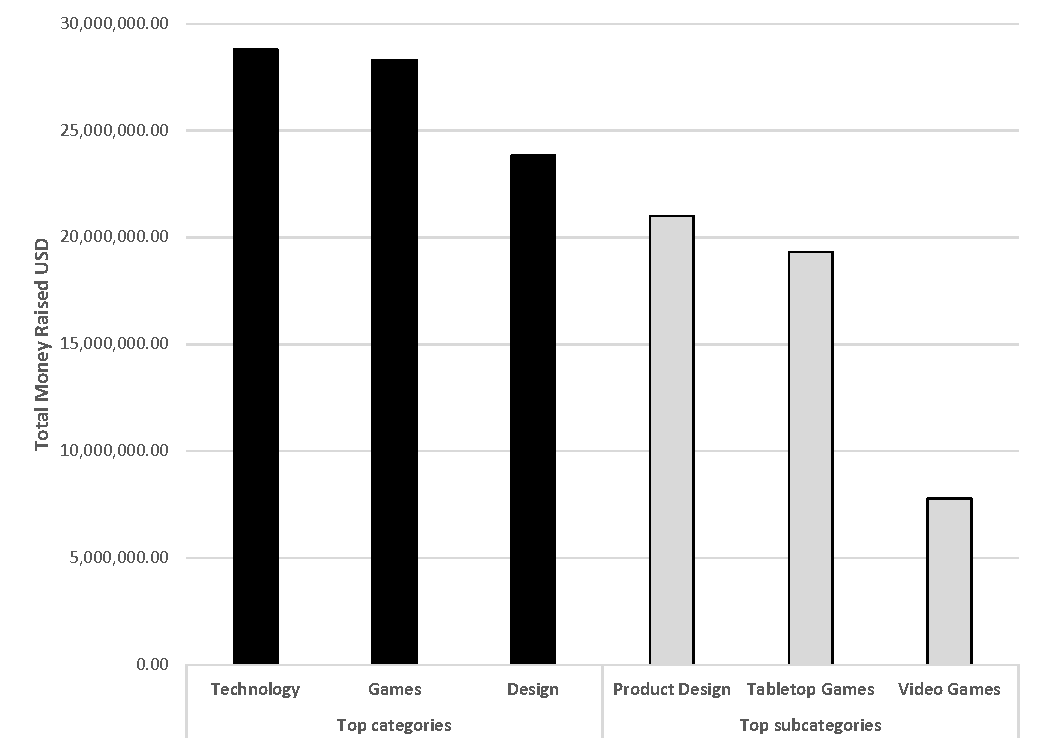
\includegraphics[width=.48\linewidth]{top-category.pdf}%
            \label{subfig:top-category}%
        }\hfill
        \subfloat[Total No. Campaigns Comparing Short vs Long Duration.]{%
            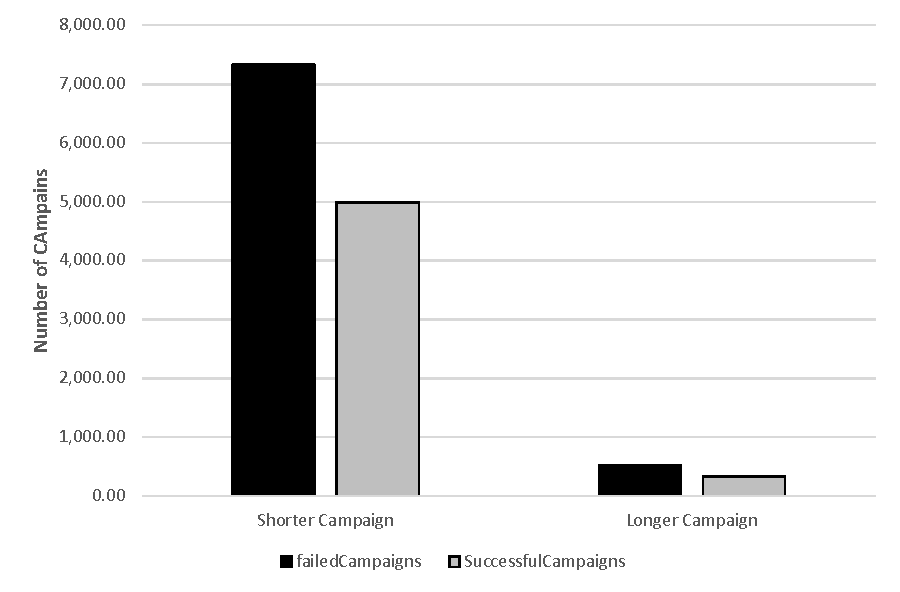
\includegraphics[width=.48\linewidth]{short_vs_long.pdf}%
            \label{subfig:short_vs_long}%
          }\\   
          \subfloat[Average Amount Pledged Comparing Short vs Long Campaigns.]{%
            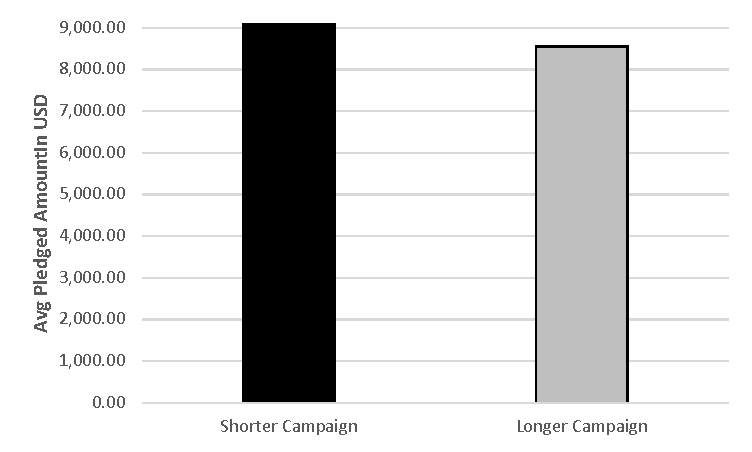
\includegraphics[width=.48\linewidth]{avg_pledge_short_long.pdf}%
            \label{subfig:avg_pledge_short_long}%
        }\hfill
        \subfloat[Total Amount Pledged Comparing Short vs Long Campaigns.]{%
            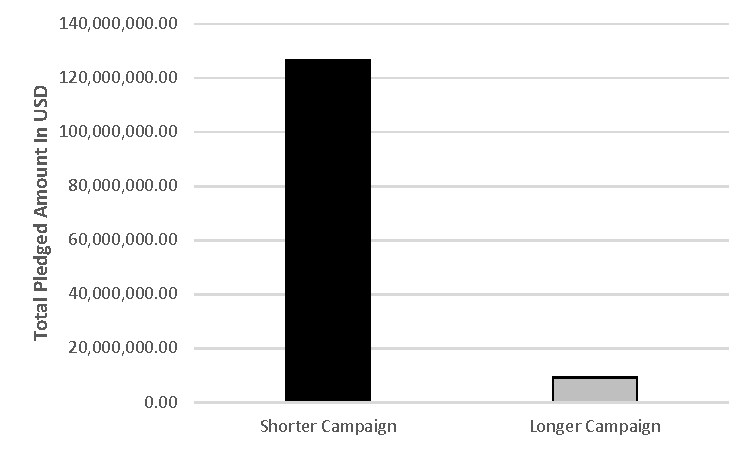
\includegraphics[width=.48\linewidth]{Avg_Pledge_Amount_USD.pdf}%
            \label{subfig:Avg_Pledge_Amount_USD}%
       } \\   
          \subfloat[Total Number of Backers.]{%
            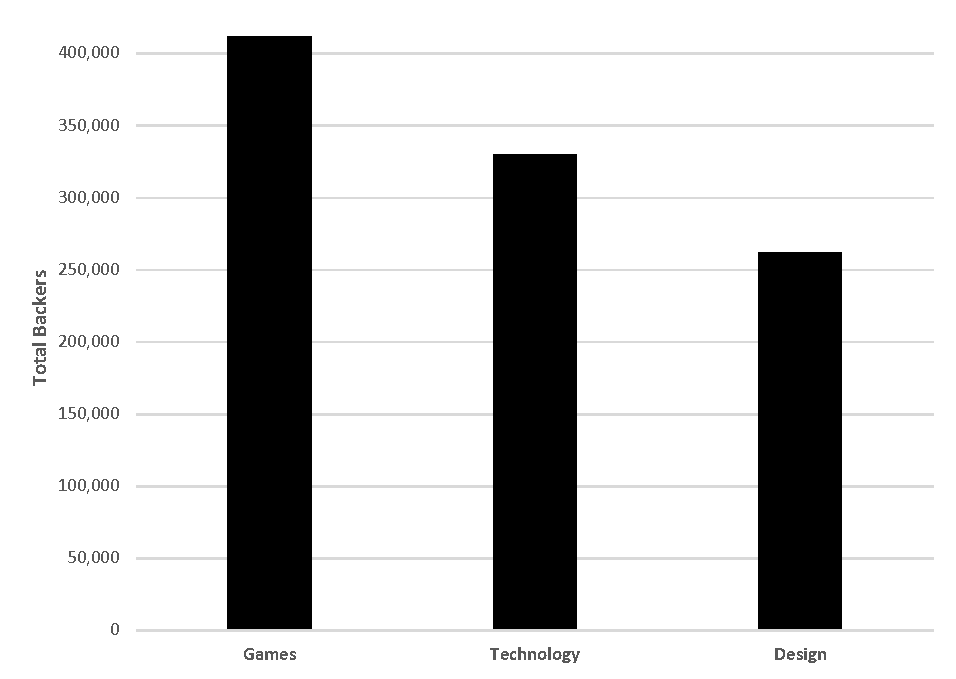
\includegraphics[width=.48\linewidth]{total_backers.pdf}%
            \label{subfig:total_backers}%
        }     
        \caption{Kickstarter Campaigns}
        \label{fig:fig}
    \end{figure*}






%\subsubsection*{Counts of words} 
%\wordcount % does not work

%%%%%%%%%%%%%%%%%%%%%%%%%%%%%%%%%%%%%%%%
%\section*{Bibliography}
%----------------------------------------------------------------------------------------
% BIBLIOGRAPHY
%----------------------------------------------------------------------------------------

%\label{Bibliography} %\lhead{\emph{Bibliography}} % Change the page header to say "Bibliography"
%\section*{Reference}
\def\bibsection{\section*{\refname}} 
\bibliography{parkour_reference} % The references (bibliography) information are stored in the file named "Bibliography.bib"


\clearpage

\end{document}